
\documentclass[a4paper, 12pt]{article} 

%--------------------------------------
%Russian-specific packages
%--------------------------------------
%\usepackage[warn]{mathtext}
\usepackage[T2A]{fontenc}
\usepackage[utf8]{inputenc}
\usepackage[english,russian]{babel}
\usepackage[intlimits]{amsmath}
\usepackage{esint}
%--------------------------------------
%Hyphenation rules
%--------------------------------------
\usepackage{hyphenat}
\hyphenation{ма-те-ма-ти-ка вос-ста-нав-ли-вать}
%--------------------------------------
%Packages
%--------------------------------------
\usepackage{amsmath}
\usepackage{amssymb}
\usepackage{amsfonts}
\usepackage{amsthm}
\usepackage{latexsym}
\usepackage{mathtools}
\usepackage{epstopdf}
\usepackage{etoolbox}%Булевые операторы
\usepackage{extsizes}%Выставление произвольного шрифта в \documentclass
\usepackage{geometry}%Разметка листа
\usepackage{indentfirst}
\usepackage{wrapfig}%Создание обтекаемых текстом объектов
\usepackage{fancyhdr}%Создание колонтитулов
\usepackage{setspace}%Настройка интерлиньяжа
\usepackage{lastpage}%Вывод номера последней страницы в документе, \lastpage
\usepackage{soul}%Изменение параметров начертания
\usepackage{hyperref}%Две строчки с настройкой гиперссылок внутри получаеммого
\usepackage[usenames,dvipsnames,svgnames,table,rgb]{xcolor}% pdf-документа
\usepackage{multicol}%Позволяет писать текст в несколько колонок
\usepackage{cite}%Работа с библиографией
\usepackage{subfigure}% Человеческая вставка нескольких картинок
\usepackage{tikz}%Рисование рисунков
\usepackage{float}
% Для картинок Моти
\usepackage{misccorr}
\usepackage{lscape}
\usepackage{cmap}


\usepackage{graphicx,xcolor}
\graphicspath{{Pictures/}}
\DeclareGraphicsExtensions{.pdf,.png,.jpg}

%----------------------------------------
%Список окружений
%----------------------------------------
\newenvironment {theor}[2]
{\smallskip \par \textbf{#1.} \textit{#2}  \par $\blacktriangleleft$}
{\flushright{$\blacktriangleright$} \medskip \par} %лемма/теорема с доказательством
\newenvironment {proofn}
{\par $\blacktriangleleft$}
{$\blacktriangleright$ \par} %доказательство
%----------------------------------------
%Список команд
%----------------------------------------
\newcommand{\grad}
{\mathop{\mathrm{grad}}\nolimits} %градиент

\newcommand{\diver}
{\mathop{\mathrm{div}}\nolimits} %дивергенция

\newcommand{\Def}[1]
{\underline{\textbf{#1}}} %определение

\newcommand{\RN}[1]
{\MakeUppercase{\romannumeral #1}} %римские цифры

\newcommand {\theornp}[2]
{\textbf{#1.} \textit{ #2} \par} %Написание леммы/теоремы без доказательства

\newcommand{\qrq}
{\ensuremath{\quad \Rightarrow \quad}} %Человеческий знак следствия

\newcommand{\qlrq}
{\ensuremath{\quad \Leftrightarrow \quad}} %Человеческий знак равносильности

\renewcommand{\phi}{\varphi} %Нормальный знак фи

\newcommand{\me}
{\ensuremath{\mathbb{E}}}

\newcommand{\md}
{\ensuremath{\mathbb{D}}}



%\renewcommand{\vec}{\overline}




%----------------------------------------
%Разметка листа
%----------------------------------------
\geometry{top = 3cm}
\geometry{bottom = 2cm}
\geometry{left = 1.5cm}
\geometry{right = 1.5cm}
%----------------------------------------
%Колонтитулы
%----------------------------------------
\pagestyle{fancy}%Создание колонтитулов
\fancyhead{}
%\fancyfoot{}
\fancyhead[R]{\textsc{ОДУ: Контрольная работа 1}}%Вставить колонтитул сюда
%----------------------------------------
%Интерлиньяж (расстояния между строчками)
%----------------------------------------
%\onehalfspacing -- интерлиньяж 1.5
%\doublespacing -- интерлиньяж 2
%----------------------------------------
%Настройка гиперссылок
%----------------------------------------
\hypersetup{				% Гиперссылки
	unicode=true,           % русские буквы в раздела PDF
	pdftitle={Заголовок},   % Заголовок
	pdfauthor={Автор},      % Автор
	pdfsubject={Тема},      % Тема
	pdfcreator={Создатель}, % Создатель
	pdfproducer={Производитель}, % Производитель
	pdfkeywords={keyword1} {key2} {key3}, % Ключевые слова
	colorlinks=true,       	% false: ссылки в рамках; true: цветные ссылки
	linkcolor=blue,          % внутренние ссылки
	citecolor=blue,        % на библиографию
	filecolor=magenta,      % на файлы
	urlcolor=cyan           % на URL
}
%----------------------------------------
%Работа с библиографией 
%----------------------------------------
\renewcommand{\refname}{Список литературы}%Изменение названия списка литературы для article
%\renewcommand{\bibname}{Список литературы}%Изменение названия списка литературы для book и report
%----------------------------------------
\begin{document}
\begin{titlepage}
\begin{center}


\vfill






\textbf{РЕШЕНИЯ ЗАДАЧ \\[3mm]
КОНТРОЛЬНОЙ РАБОТЫ №1\\[3mm]
по курсу "Обыкновенные дифференциальные уравнения"
\\[20mm]
}
\end{center}


\tableofcontents

\end{titlepage}

\newpage




	\section{Вариант I}
		\subsection {Задача 1}


Уравнение:
\begin{equation}
\dot{x}=\frac{\sqrt{1-x^2}}{x}, \;\;\;\;\; x( \cdot ) \in \bf{R}
\end{equation}

(i) Из условия $\dot{x}=0 \Rightarrow x=\pm 1$ - стационарные решения. 
\[D = R \times \{1-x^2\geq 0, x \neq 0\} \]
По теореме Пеано решения существуют.

(ii) Для задачи Коши с $x(0)=1/2$:
\[f(x, t) := \frac{\sqrt{1-x^2}}{x}\]
$\frac {df}{dx}$ непрерывна на $D \backslash \{x^2=1\} \; \Rightarrow $ для этих начальных данных решение единственно. 

(iii) Интегрируя (1) и используя метод разделения переменных (с учетом начальных условий), получаем уравнение: 

\begin{equation}
	-\sqrt{1-x^2} = t - \sqrt{3}/2
\end{equation}

Проведем некоторые преобразования. Тогда из (2):
\[ x = \pm \sqrt{-t^2+\sqrt{3}t+1/4}, \;\;\;\;\;\; t\leq \sqrt{3}/2\]
Легко проверить, что для наших начальных данных нужно брать решение  с +.


Общее решение задачи Коши:
\begin{equation*}
x(t) = 
 \begin{cases}
   \sqrt{-t^2+\sqrt{3}t+1/4}, \;\;\;\;\;\;  -1+\sqrt{3}/2 < t\leq \sqrt{3}/2\\
   1, \;\;\;\;\;\; t\geq \sqrt{3}/2
 \end{cases}
\end{equation*}


(iv)-(v) Максимальные интервалы существования решений.\\
В (2) обозначим левую часть за G(x), правую -- за F(t).
 
\begin{figure}[H]
	\centering
	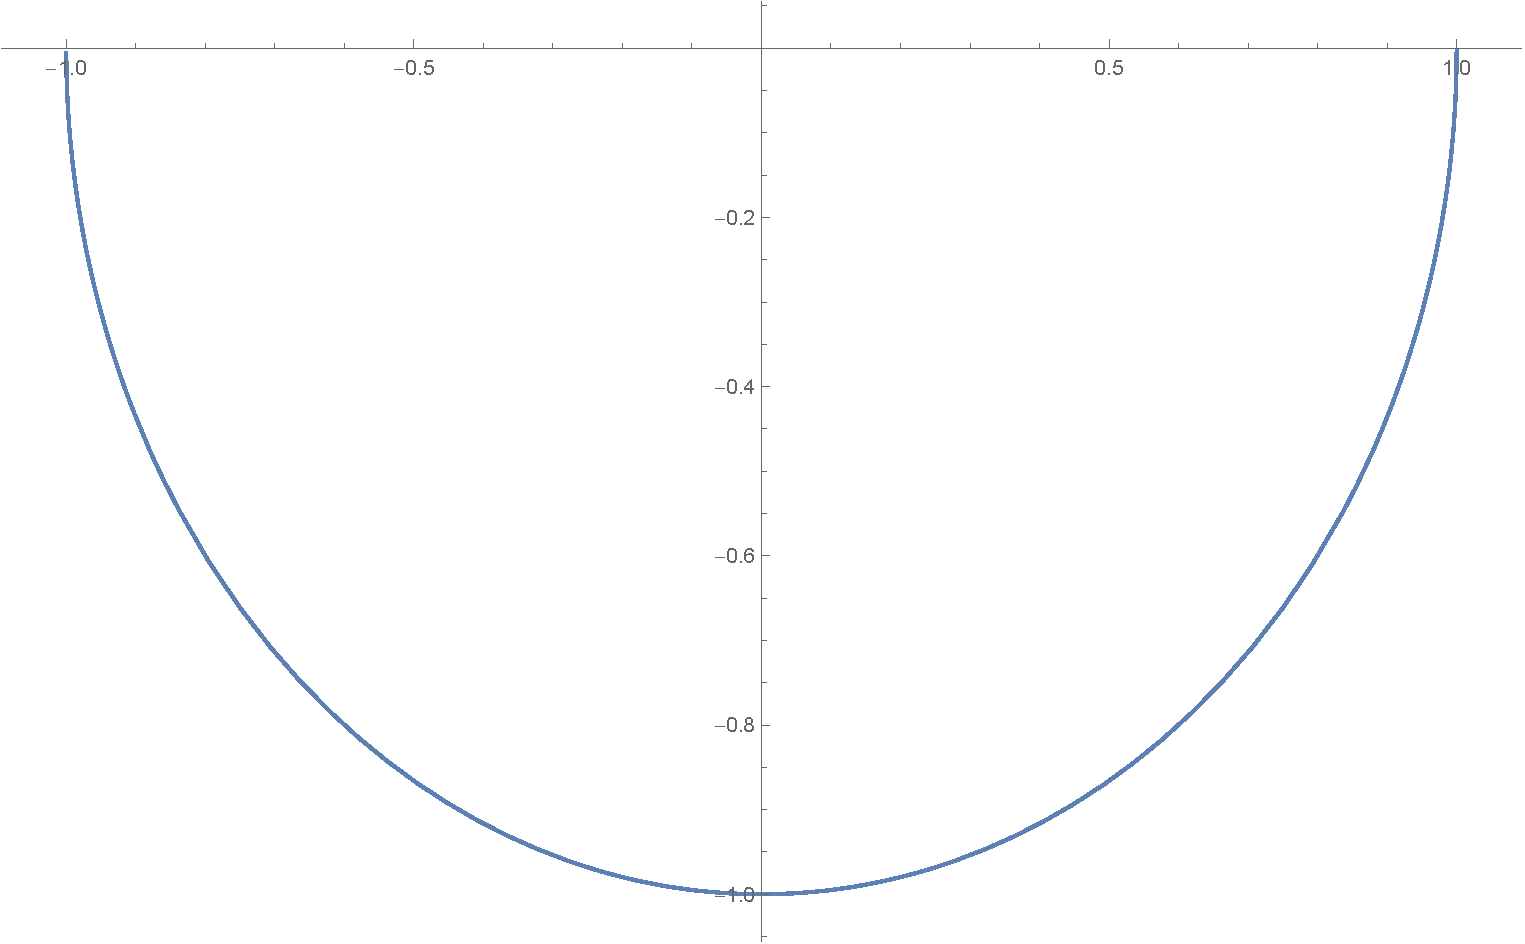
\includegraphics[scale=0.6]{1}
	\caption{G(x)}
\end{figure}
F(t) должна принадлежать прообразу G(x), т.е.:
\[-1+\sqrt{3}/2 < t \leq \sqrt{3}/2 \]
Считая пределы в крайних точках, найдем значение x:
\[\lim_{t \rightarrow -1+\sqrt{3}/2} x(t) = \pm \sqrt{-(-1+\sqrt{3}/2)^2+\sqrt{3}(-1+\sqrt{3}/2)+1/4} = 0\]
\[\lim_{t  \rightarrow \sqrt{3}/2} x(t) = \pm \sqrt{-(\sqrt{3}/2)^2+\sqrt{3}(\sqrt{3}/2)+1/4} = \pm 1\]

Также найдем значение производной $\dot{x}$ в этих точках:

\[\lim_{x  \rightarrow 0}\dot{x(t)} = +\infty\]
\[\lim_{x  \rightarrow \pm 1 }\dot{x(t)} = 0\]
Т. о. при $t = \sqrt{3}/2$  доопределяем решение (2) решением $+1$ и получаем решение задачи Коши:

\begin{equation*}
x(t) = 
 \begin{cases}
   \sqrt{-t^2+\sqrt{3}t+1/4}, \;\;\;\;\;\;  -1+\sqrt{3}/2 < t\leq \sqrt{3}/2\\
   1, \;\;\;\;\;\; t\geq \sqrt{3}/2
 \end{cases}
\end{equation*}



Максимальный интервал существования решения: $(-1+ \sqrt{3}/2; +\infty)$

(vi) Интервалы монотонности, точки максимумов и минимумов:

\[\dot{x}=\frac{\sqrt{1-x^2}}{x}\]
\[ x < 0: \dot{x}  \geq 0\]
\[x > 0: \dot{x} \leq 0\]
Также найдем промежутки выпуклости функции:
\[ \ddot{x} = -1/x^3\]
\[ x > 0: \ddot{x} \geq 0\]
\[x < 0: \ddot{x} \leq 0\]

Кривая, проходящая через (0, 1/2) не убывает на  $(-1+ \sqrt{3}/2; +\infty)$.
Точки минимума и максимума (локальные = глобальные):
\[x_{max} = 1, \;\;\;\;\; x_{min}= -1\]
(vii) График решения:
(Красная линия -- прямая $x=0$, которая исключена из D.)




Наше решение: верхняя ветвь полуокружности, входящая в x = 1.

\begin{figure}[H]
	\centering
	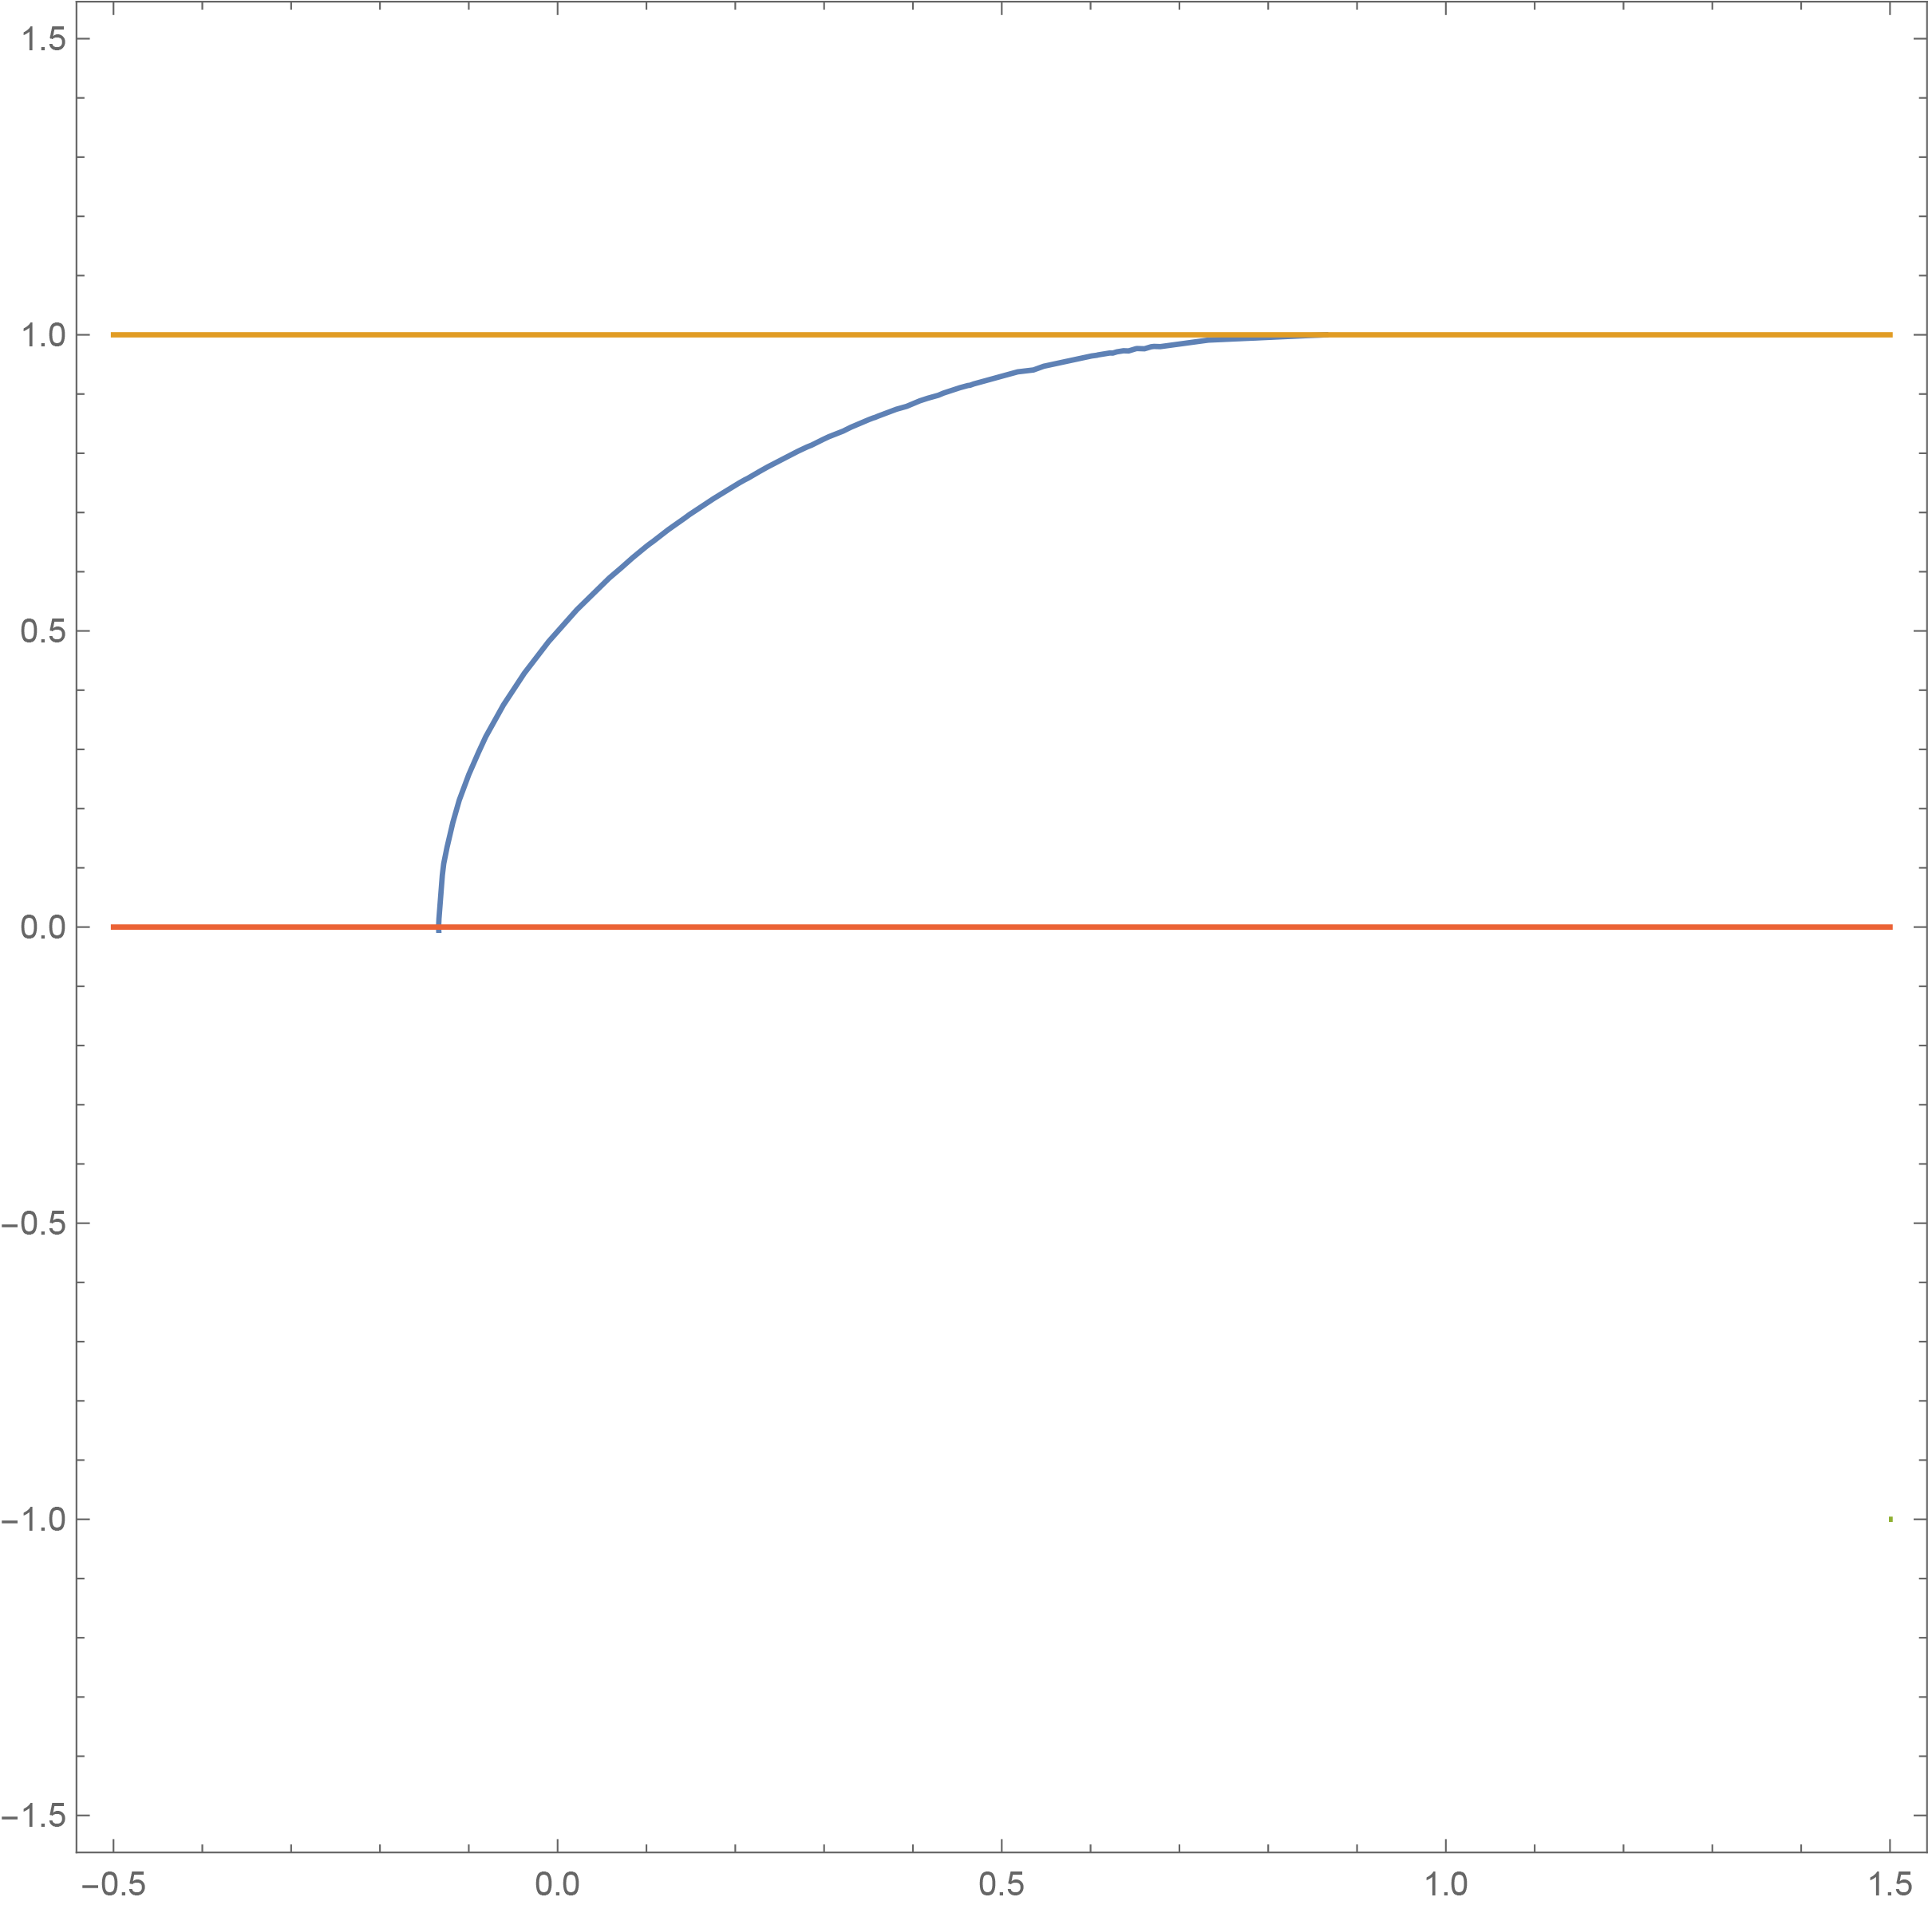
\includegraphics[scale=0.47]{2.png}
	\caption{Решение ДУ (1) с учетом начальных условий $(0, 1/2)$}
\end{figure}




	\subsection {Задача 2}



Задача Коши 
\begin{equation}
y'+xy=e^x,\;\;\;\;\;\;y(-1) = 1, \;\;\;\;\;\;y(\cdot) \in \bf{R}
\end{equation}


(i) Решение и единственность:\\
Область определения: $D = R\times R$. По т. Пеано решения существуют. 
\[f(y, x) = e^x-yx, \;\;\;\; \frac{df}{dy} = - x\;\; \text{непрерывна на D, решения единственны.}\]
Метод решения линейных ДУ: представление функции y(x) как произведение двух других:
\[y=uv, \;\;\;\;\;\;y'=u'v+uv'\]
Подставляя в (3), находим:
\[u'v+uv'+uvx=e^x\]
Пусть
\[v'+vx=0\]
Тогда
\[v= e^{-\frac{x^2} 2}\]
\[u=\int_{-1}^x e^{s^2/2+s} ds+ c= e^{-1/2} \int_{-1}^{x} e^{s^2/2+s+1/2} ds+c = e^{-1/2}\int_0^{(x+1)} e^{t^2/2} dt+c\]
	\[y = uv = e^{-\frac{x^2} 2}  e^{-1/2}\int_{0}^{(x+1)} e^{t^2/2} dt+ce^{-\frac{x^2} 2}\] 
Найдем константу:
\[y(-1)=ce^{-1/2}=1\;\;\;\;\;\; c = e^{1/2}\]
Тогда решение имеет вид:
\[y =e^{-\frac{x^2} 2- \frac 1 2 } \int_{0}^{(x+1)} e^{t^2/2} dt+e^{-\frac{x^2} 2 +\frac 1 2 }\] 

(ii) Решения определены на всей вещественной оси.

(iii) Предел на бесконечности:
\[ \lim_{x\rightarrow +\infty} \frac  {\int_{0}^{(x+1)} e^{t^2/2} dt} {e^{\frac{x^2} 2 + \frac 1 2 }}+\]
\[+e^{-\frac{x^2} 2 +\frac 1 2 }= \frac  {e^{(x^2+2x+1)/ 2}} {2x e^{\frac{x^2} 2 + \frac 1 2 }} = +\infty \;\;\text{Лопиталь}\]

\[\lim_{x\rightarrow -\infty} \frac  {\int_{0}^{(x+1)} e^{t^2/2} dt} {e^{\frac{x^2} 2 + \frac 1 2 }}+e^{-\frac{x^2} 2 +\frac 1 2 }=\lim_{x\rightarrow -\infty} \frac  {e^{(x^2+2x+1)/ 2}} {2x e^{\frac{x^2} 2 + \frac 1 2 }} = 0\]

(iv) График решения:\\
Знаки производной:
\[y' > 0,\;\;\;\;\; e^x-xy>0\]
\[xy<e^x\]
\[
\left[ 
  \begin{gathered} 
    \left\{ 
      \begin{gathered} 
        x  > 0
        \\ 
        y < \frac {e^x} {x}
        \\
      \end{gathered} 
    \right.  
    \\ 
    \left\{ 
      \begin{gathered} 
        x  < 0
        \\ 
        y > \frac {e^x} {x}
        \\
      \end{gathered} 
    \right.
    \\
  \end{gathered}
\right.
\]
\begin{figure}[H]
	\centering
	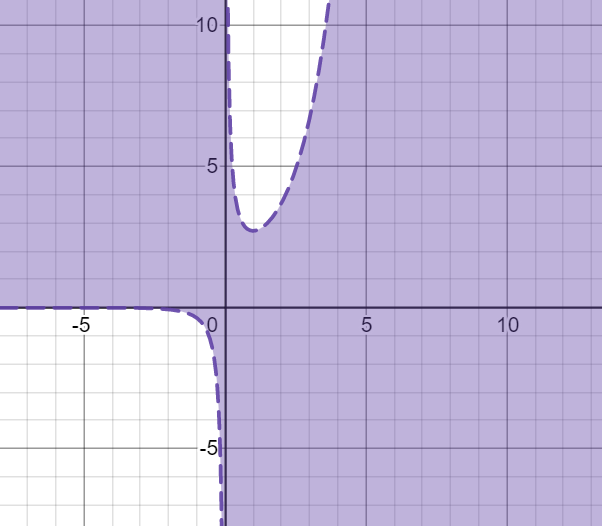
\includegraphics[scale=0.5]{11}
	\caption{Знаки производной (функция возрастает в закрашенной области)}
\end{figure}

Решение $y =e^{-\frac{x^2} 2- \frac 1 2 } \int_{0}^{(x+1)/ \sqrt{2}} e^{t^2} dt+e^{-\frac{x^2} 2 +\frac 1 2 }$ монотонно возрастает на $\bf{R}.$

\begin{figure}[H]
	\centering
	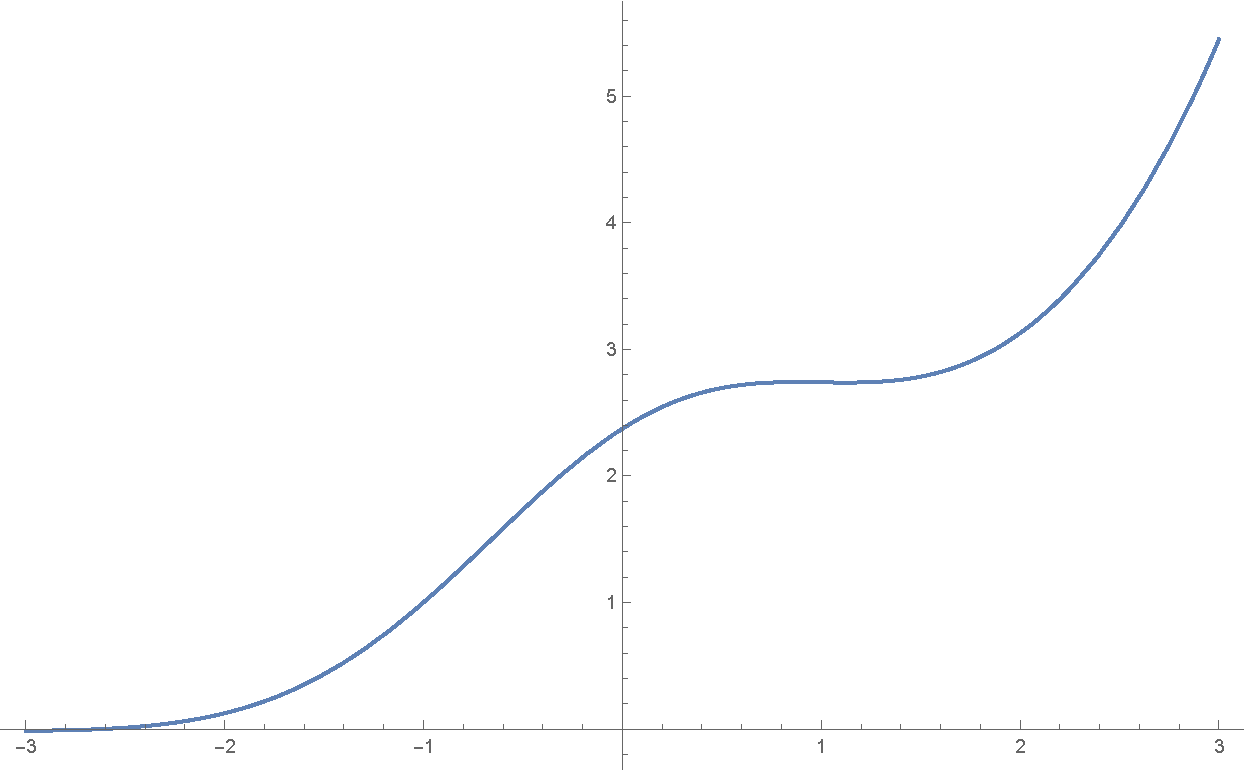
\includegraphics[scale=0.7]{17}
	\caption{Решение задачи Коши (3)}
\end{figure}


\begin{figure}[H]
	\centering
	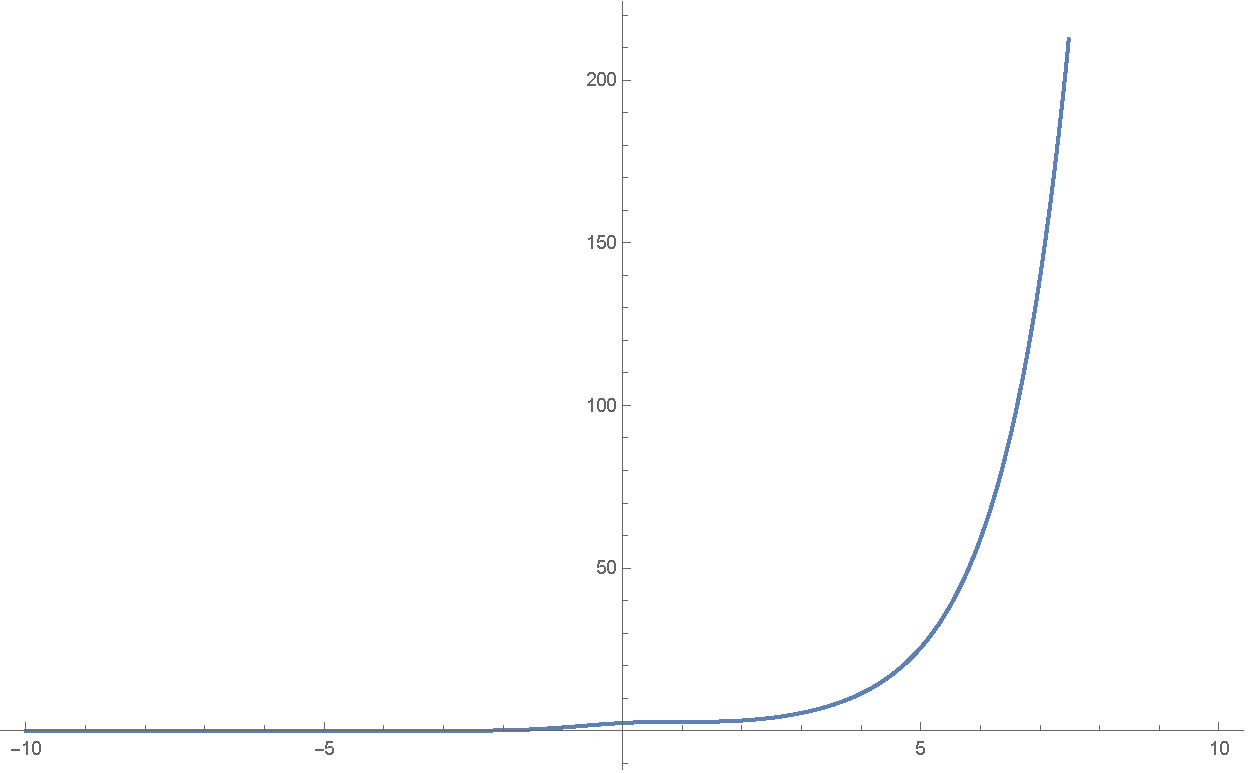
\includegraphics[scale=0.7]{12}
	\caption{Решение задачи Коши (3)}
\end{figure}

		\subsection {Задача 3}


\begin{equation}
(y-x)y'=y, \;\;\;\;\;\;y(\cdot) \in \bf{R}
\end{equation}

(i) $D = R \times R$. Разделим уравнение на (y-x) (это законно, т.к. прямая x=y не может быть решением (4) с нашими начальными условиями). Для нач. условий (0, 1) (4) эквивалентно следующему уравнению:
 \[y'=\frac {y}{(y-x)}\]
Левая часть непрерывно дифф-ма, на $D\backslash \{y=x\}$, следовательно, есть только одна траектория, проходящая через (0, 1).  Найдем ее.

Предположение: наше уравнение является полным дифференциалом какой-то функции.
\[dy(y-x)-dx\cdot y= 0\]
\[f = f'_xdx+f'_ydy\]
\[f'_y=y-x\;\;\;\;\;\;\;\;\;\;\;\; f'_x=-y\]
\[f''_{y, x}=-1\;\;\;\;\;\;\;\;\;\;\;\; f''_{x, y}=-1\]
\[f''_{y, x}=f''_{x, y}\]
Сошлось. Тогда:
\[f = xy+C(y)\]
\[f'(y)=x+C'(y)=y-x\]
\[C'(y)=y-2x\]
\[C(y)=\frac{y^2}{2}-2xy+C\]
\[f= \frac{y^2}{2}-2xy+C=0\]
\[C=-\frac 1 2 \]
\[y^2-2xy-1+x^2=x^2\]
\[y =  \sqrt{x^2+1}+x\]

(ii) Максимальный интервал существования решения -- вся вещественная ось. 

(iii)Найдем асимптоты  нашей кривой:
\[ \sqrt{x^2+1}+x = o(1) \quad \quad \text{при $x \rightarrow - \infty$}\]
\[ \sqrt{x^2+1}+x = 2x + o(1) \quad \quad \text{при $x \rightarrow + \infty$}\]

(iv) Интервалы монотонности и график траектории:
Знаки производной:
\[y' > 0,\;\;\;\;\; \frac y {y-x}>0\]
\[
\left[ 
  \begin{gathered} 
    \left\{ 
      \begin{gathered} 
        y  > 0
        \\ 
        y - x > 0
        \\
      \end{gathered} 
    \right.  
    \\ 
    \left\{ 
      \begin{gathered} 
        y  < 0
        \\ 
        y - x < 0
        \\
      \end{gathered} 
    \right.
    \\
  \end{gathered}
\right.
\]

\begin{figure}[H]
	\centering
	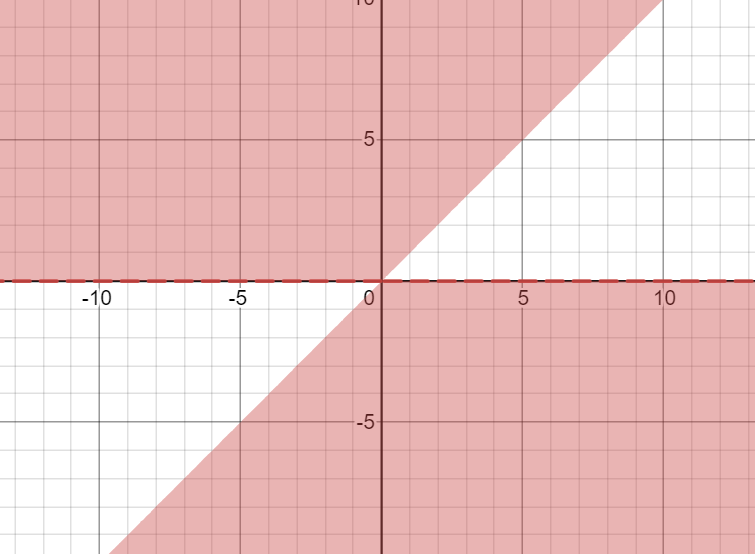
\includegraphics[scale=0.6]{9}
	\caption{Знаки производной (функция возрастает в закрашенной области)}
\end{figure}

Интервалы монотонности:\\
Решение (4) монотонно возрастает на $\bf{R}$.

\begin{figure}[H]
	\centering
	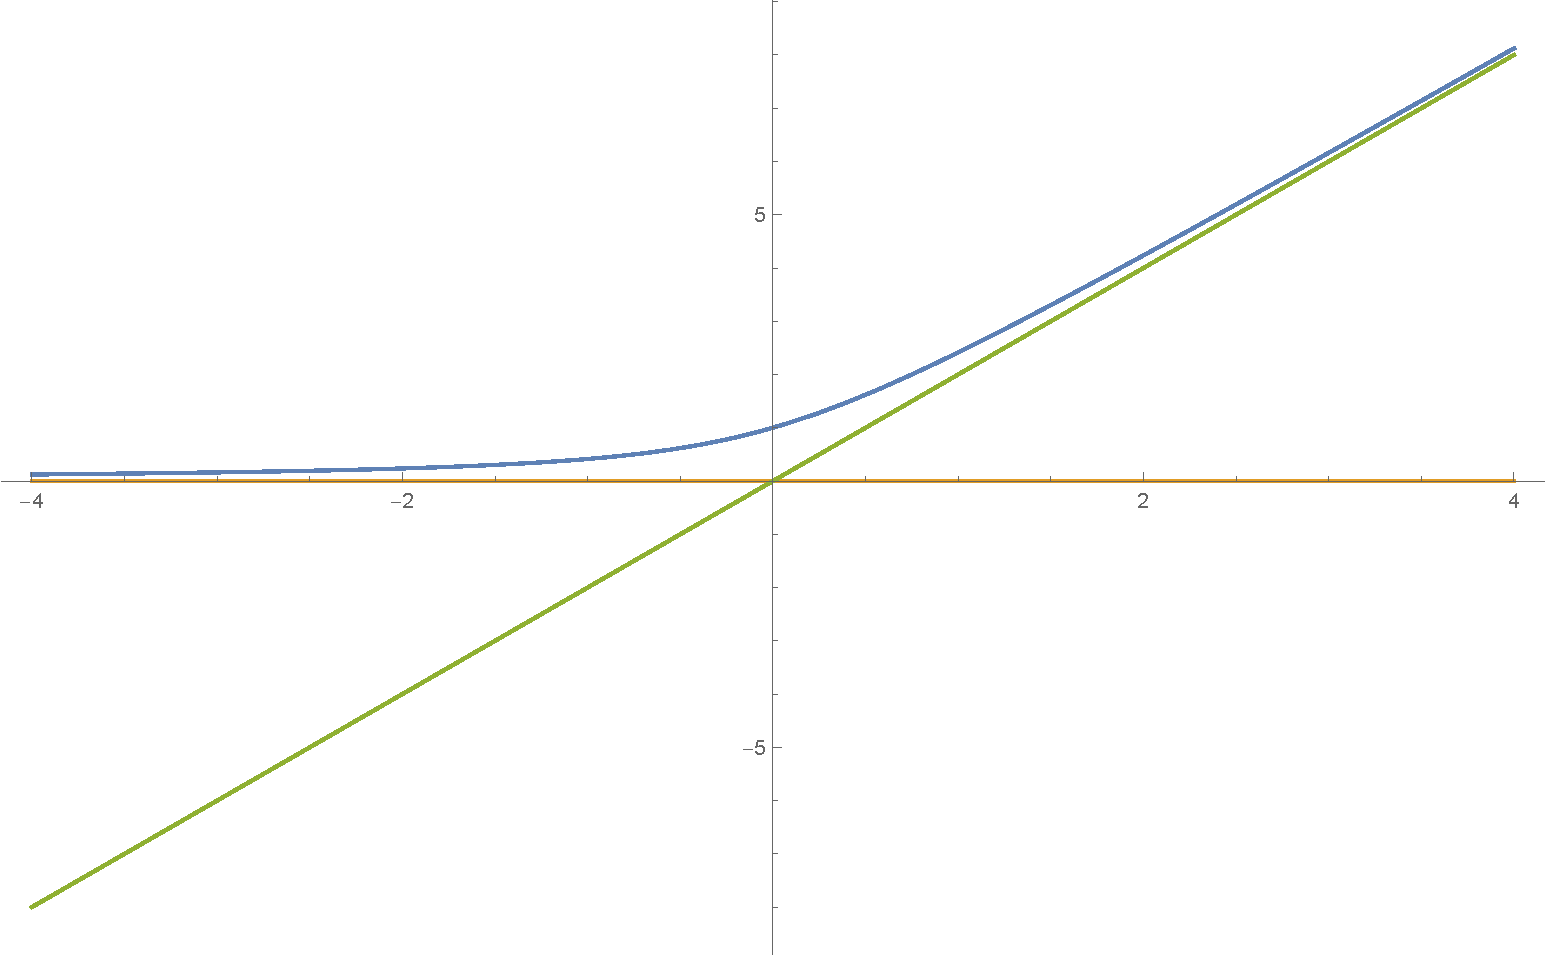
\includegraphics[scale=0.6]{4}
	\caption{Решение ДУ (4) с учетом начальных условий $(0, -1)$}
\end{figure}




	\section{Вариант II}


		\subsection {Задача 1}


Уравнение:
\begin{equation}
\dot{x}=-\frac{\sqrt{1-x^2}}{2}, \;\;\;\;\; x( \cdot ) \in \bf{R}
\end{equation}

(i) Из условия $\dot{x}=0 \Rightarrow x=\pm 1$ - стационарные решения. 
\[D = R \times \{1-x^2\geq 0\} \]

(ii) Для задачи Коши с $x(0)=1/2$:
\[f(x, t) :=- \frac{\sqrt{1-x^2}}{2}\]
$\frac {df}{dx}$ непрерывна на $D \backslash \{x^2=1\} \; \Rightarrow $ для  начальных данных из этого мн-ва решение единственно, По теореме Пеано решения существуют для всех начальных данных.

(iii) Интегрируя (5) и используя метод разделения переменных (с учетом начальных условий), получаем уравнение: 

\begin{equation}
	-\arcsin(x) = \frac t 2 - \frac {\pi}{6}
\end{equation}


Общее решение задачи Коши:
\begin{equation*}
x(t) = 
 \begin{cases}
    1, \;\;\;\;\;\; t\leq -\frac{2\pi}3\\
   \sin( -\frac t 2 + \frac {\pi}{6}), \;\;\;\;\;\;  -\frac{2\pi}3 \geq  t\geq \frac{4\pi}3\\
   -1, \;\;\;\;\;\; t\geq \frac{4\pi}3
 \end{cases}
\end{equation*}



(iv)-(v) Максимальные интервалы существования решений.\\
В (2) обозначим левую часть за G(x), правую -- за F(t).
 
\begin{figure}[H]
	\centering
	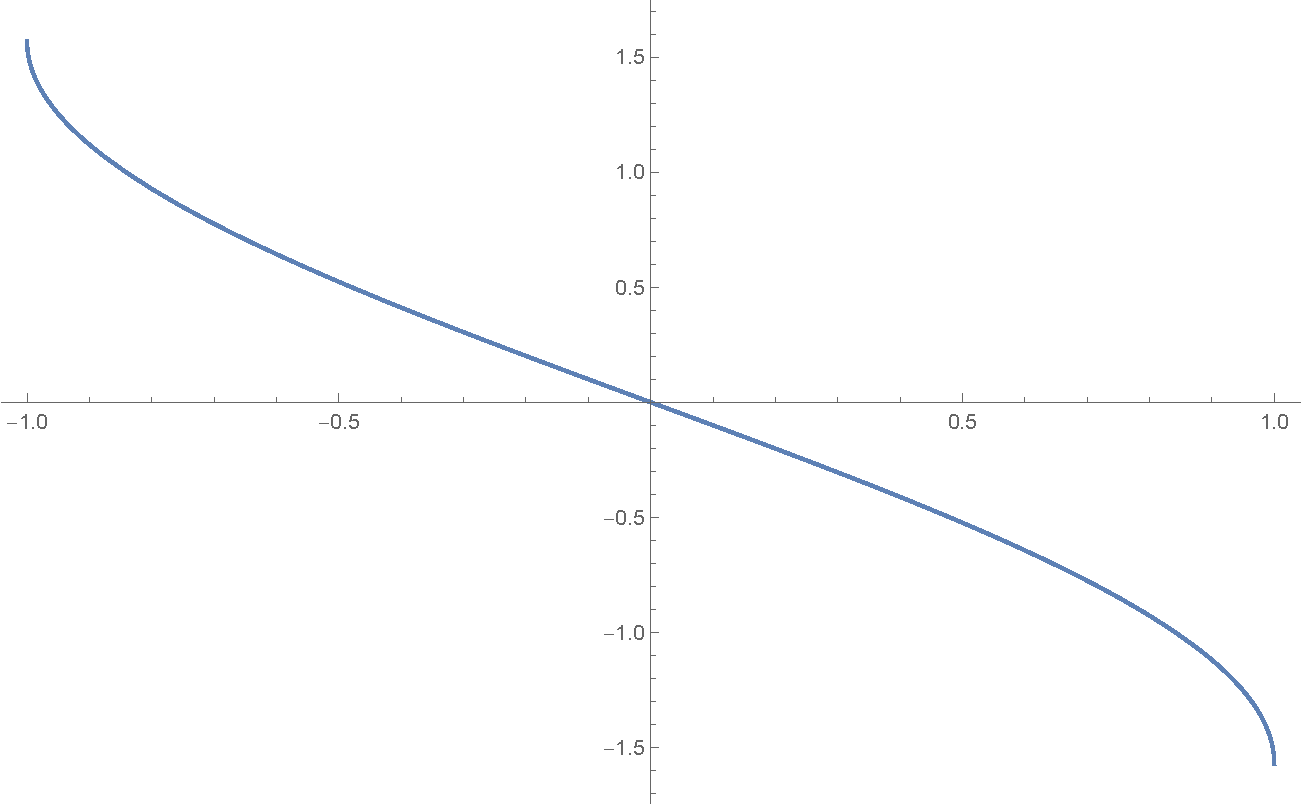
\includegraphics[scale=0.6]{6}
	\caption{$G(x)=-\arcsin(x)$}
\end{figure}
F(t) должна принадлежать прообразу G(x), т.е.:
\[\frac t 2 - \frac{\pi} 6 \in \left[-\frac{\pi} 2 , \frac{\pi} 2  \right] \]
\[\ t  \in \left[-\frac{2\pi}3 , \frac{4\pi} 3  \right] \]
Считая пределы в крайних точках, найдем значение x:
\[\lim_{t \rightarrow -\frac{2\pi}3} x(t) = \sin\left( -\frac t 2 + \frac {\pi}{6}\right) = 1\]
\[\lim_{t  \rightarrow \frac{4\pi}3} x(t) = \sin\left( -\frac t 2 + \frac {\pi}{6}\right) = -1\]

Также найдем значение производной $\dot{x}$ в этих точках:

\[\lim_{x \rightarrow -1}\dot{x(t)} = 0\]
\[\lim_{x  \rightarrow + 1 }\dot{x(t)} = 0\]

Доопределяем решение (6) в точках $ -\frac{2\pi}3 $ и $ \frac{4\pi} 3 $ решениями $\pm 1$, и получаем решение задачи Коши:

\begin{equation*}
x(t) = 
 \begin{cases}
    1, \;\;\;\;\;\; t\leq -\frac{2\pi}3\\
   \sin( -\frac t 2 + \frac {\pi}{6}), \;\;\;\;\;\;  -\frac{2\pi}3 \geq  t\geq \frac{4\pi}3\\
   -1, \;\;\;\;\;\; t\geq \frac{4\pi}3
 \end{cases}
\end{equation*}


Т. о. максимальный интервал существования решения: $(-\infty; +\infty)$

(vi) Интервалы монотонности, точки максимумов и минимумов:

\[\dot{x}=-\frac{\sqrt{1-x^2}}{2}\]

\[ 0 \geq \dot{x} \; \text{на D}\]
Также найдем промежутки выпуклости функции:
\[ \ddot{x} = x/4\]
\[ x < 0: \ddot{x} \geq 0 \]
\[x > 0: \ddot{x} \leq 0  \]

Решение (5) монотонно не возрастает на $\bf{R}$.


Точки минимума и максимума (локальные и глобальные):
\[x_{max} = 1, \;\;\;\;\; x_{min}= -1\]
(vii) График решения:




\begin{figure}[H]
	\centering
	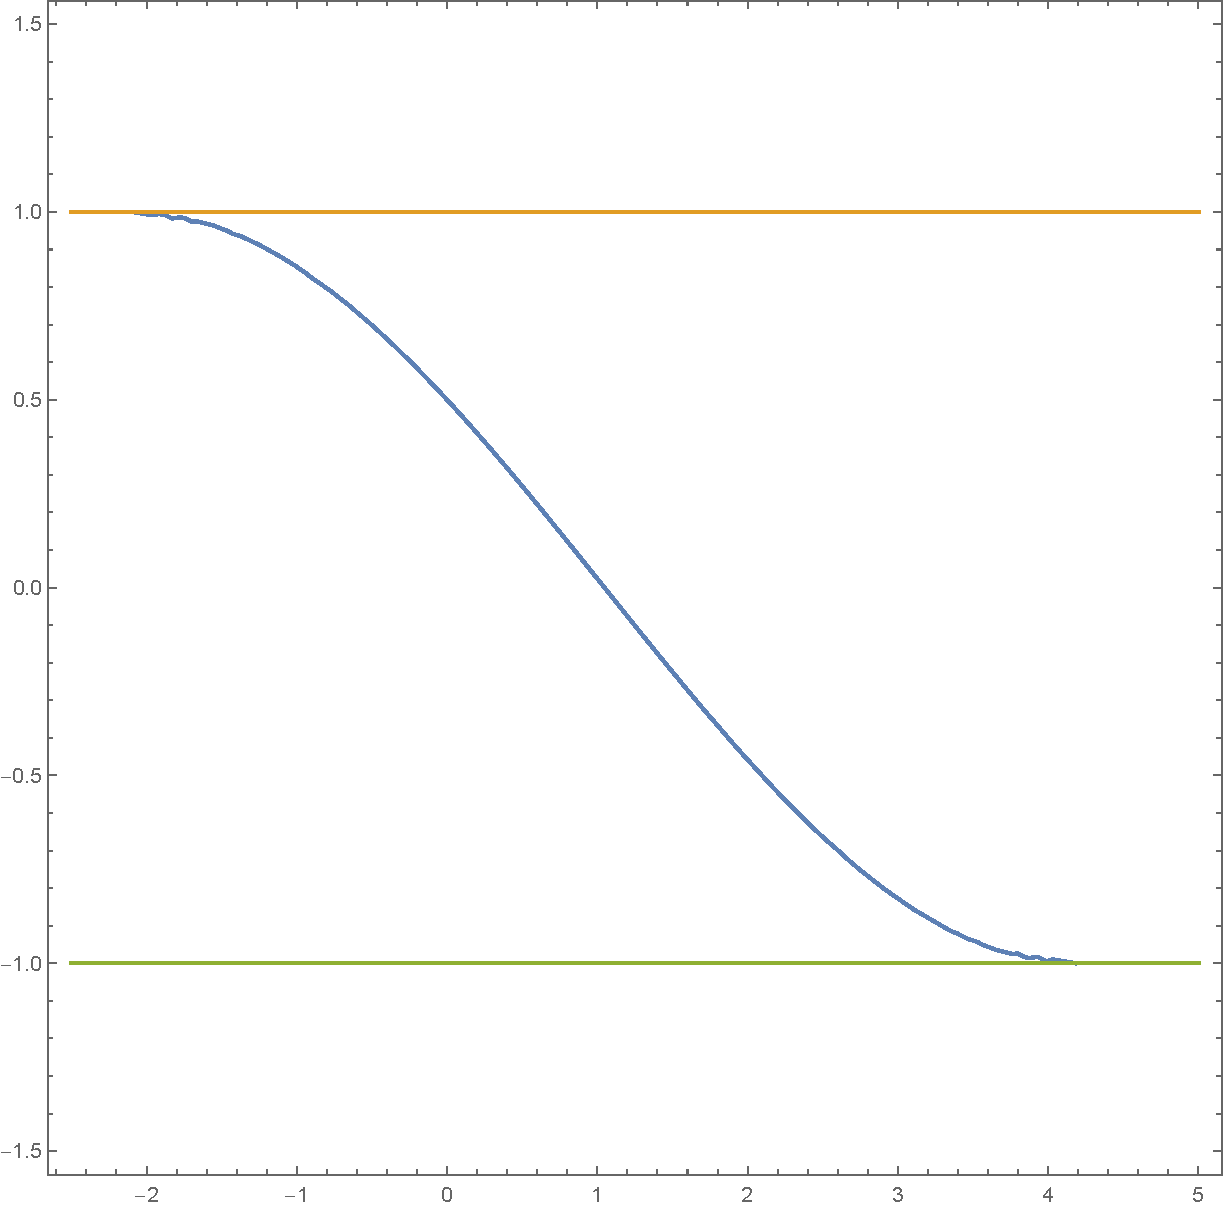
\includegraphics[scale=0.6]{7}
	\caption{Решение ДУ (1) с учетом начальных условий $(0, 1/2)$}
\end{figure}

	\subsection {Задача 2}

Задача Коши 
\begin{equation}
	y'+xy=e^{-x},\;\;\;\;\;\;y(1) = 1, \;\;\;\;\;\;y(\cdot) \in \bf{R}
\end{equation}
Решение полностью аналогично решению №2 варианта I.


\[v= e^{-\frac{x^2} 2}\]
\[u=\int_{-1}^x e^{s^2/2-s} ds+ c= e^{-1/2} \int_{-1}^{x} e^{s^2/2-s+1/2} ds+c = e^{-1/2}\int_0^{(x-1)} e^{t^2/2} dt+c\]
\[y = uv = e^{-\frac{x^2} 2}  e^{-1/2}\int_{0}^{(x-1)} e^{t^2/2} dt+ce^{-\frac{x^2} 2}\] 
Найдем константу C:
\[y(1)=Ce^{-1/2}=1\;\;\;\;\;\; C = e^{1/2}\]
Тогда решение имеет вид:
\[y =e^{-\frac{x^2} 2- \frac 1 2 } \int_{0}^{(x-1)} e^{t^2/2} dt+e^{-\frac{x^2} 2 +\frac 1 2 }\] 

(iii) Предел на бесконечности:
\[ \lim_{x\rightarrow +\infty} \frac  {\int_{0}^{(x-1)} e^{t^2/2} dt} {e^{\frac{x^2} 2 + \frac 1 2 }}+\]
\[+e^{-\frac{x^2} 2 +\frac 1 2 }=  \lim_{x\rightarrow +\infty} \frac  {e^{(x^2-2x+1)/ 2}} {2x e^{\frac{x^2} 2 + \frac 1 2 }} = 0 \;\;\text{ по правилу Лопиталя}\]

\[\lim_{x\rightarrow -\infty} \frac  {\int_{0}^{(x-1)} e^{t^2/2} dt} {e^{\frac{x^2} 2 + \frac 1 2 }}+e^{-\frac{x^2} 2 +\frac 1 2 }= \lim_{x\rightarrow -\infty} \frac  {e^{(x^2-2x+1)/ 2}} {2x e^{\frac{x^2} 2 + \frac 1 2 }} = -\infty\]

(iv) График решения:\\




\begin{figure}[H]
	\centering
	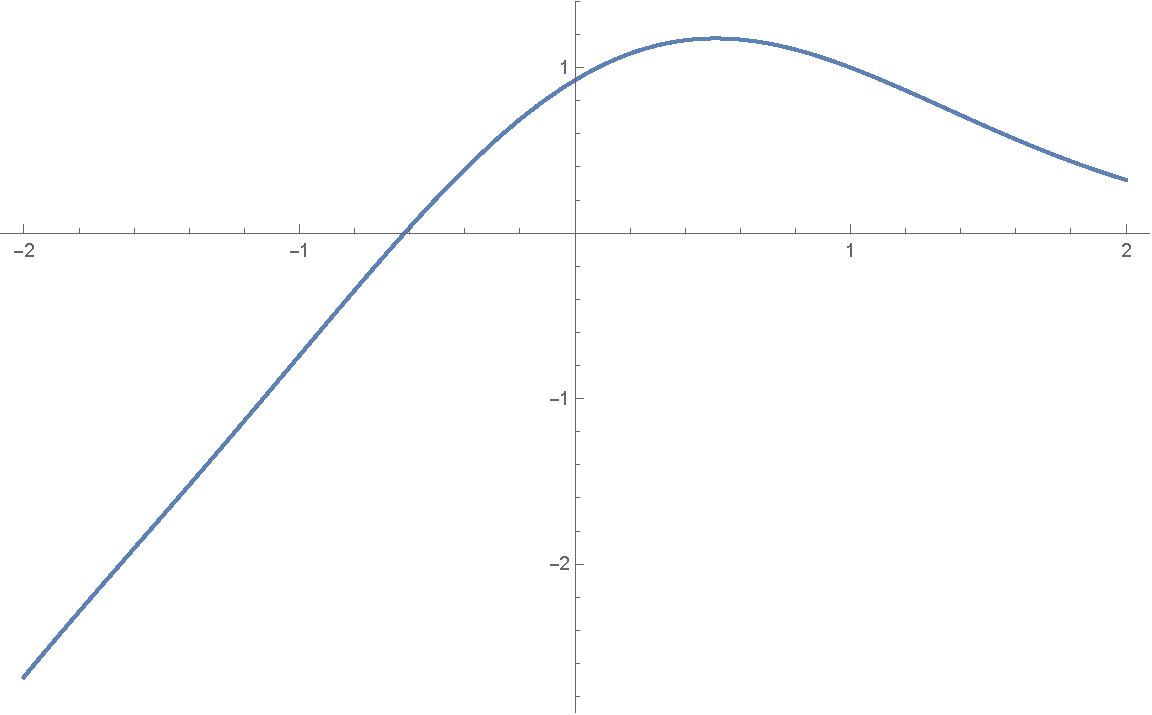
\includegraphics[scale=0.7]{16}
	\caption{Решение задачи Коши (7)}
\end{figure}

\begin{figure}[H]
	\centering
	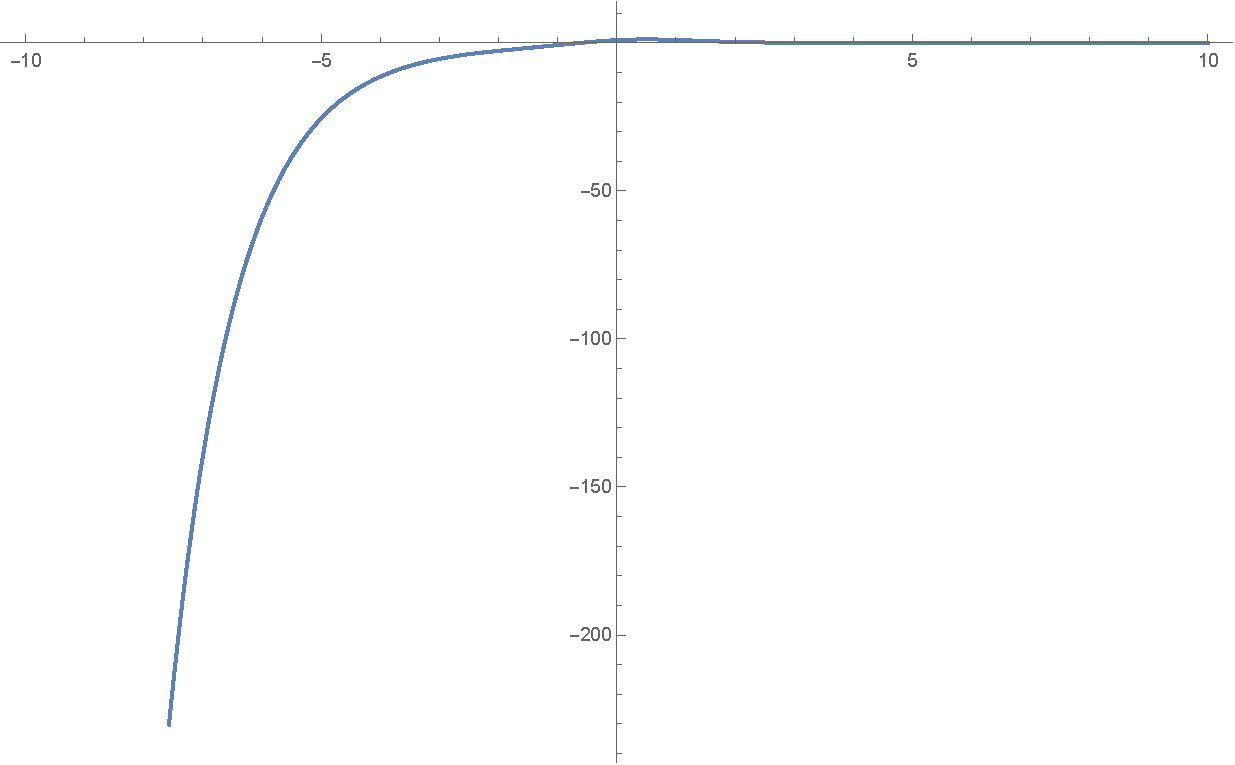
\includegraphics[scale=0.7]{13}
	\caption{Решение задачи Коши (7)}
\end{figure}

		\subsection {Задача 3}
\begin{equation}
(y-x)y'=y, \;\;\;\;\;\;y(\cdot) \in \bf{R}
\end{equation}

Решение полностью аналогично решению №3 варианта I. Для начальных условий $(0, -1)$ получаем траекторию:
\[y = - \sqrt{x^2+1}+x\]


(iii) Найдем асимптоты  нашей кривой:

\[ -\sqrt{x^2+1}+x = o(1) \quad \quad \text{при $x \rightarrow + \infty$}\]
\[ -\sqrt{x^2+1}+x = 2x + o(1) \quad \quad \text{при $x \rightarrow - \infty$}\]

\begin{figure}[H]
	\centering
	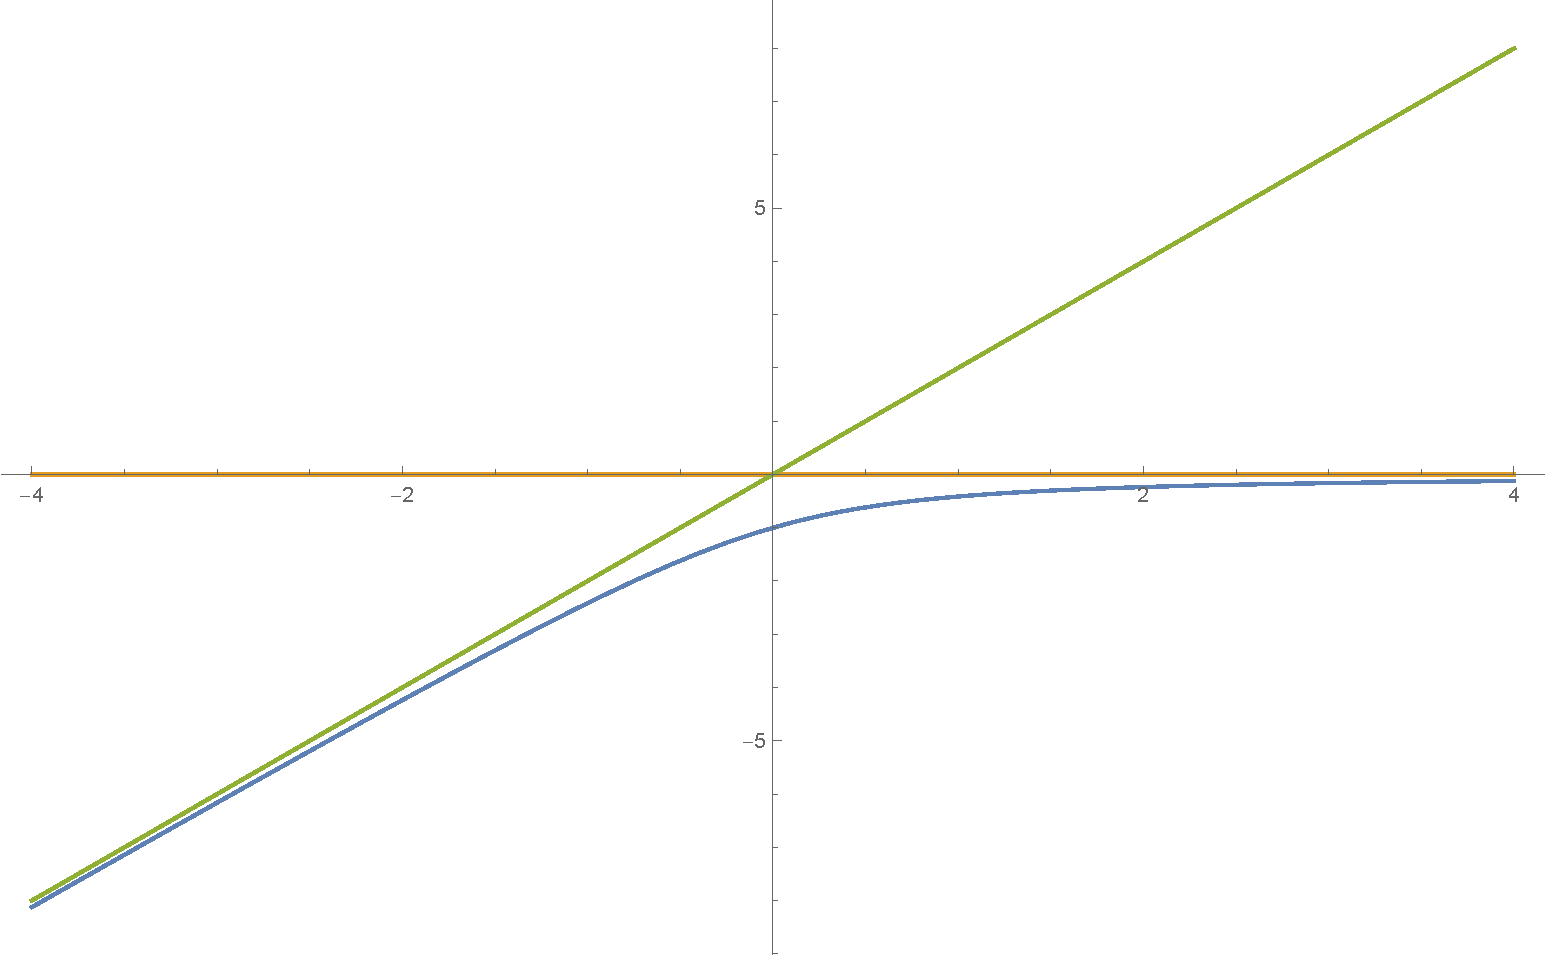
\includegraphics[scale=0.6]{5}
	\caption{Решение ДУ (4) с учетом начальных условий $(0, -1)$}
\end{figure}

	\section{Вариант III}
		\subsection {Задача 1}

Решение задачи 1 варианта III аналогично решению задачи 1 варианта I. Решение для начальных данных $x(0)=-2/3$:
\[-\sqrt{1-x^2} = t - \sqrt{5}/3\]
Максимальный интервал существования решения: $(-1+ \sqrt{5}/3; +\infty)$.\\
График решения для этих начальных данных:

Общее решение задачи Коши:
\begin{equation*}
x(t) = 
 \begin{cases}
   -\frac 1 3 \sqrt{(4+6\sqrt{5}t-9t^{2})}, \;\;\;\;\;\; -1+ \sqrt{5}/3 < t \leq \sqrt{5}/3\\
   -1, \;\;\;\;\;\; t\geq \sqrt{5}/3
 \end{cases}
\end{equation*}


Наше решение: нижняя ветвь полуокружности, входящая в x = -1.

\begin{figure}[H]
	\centering
	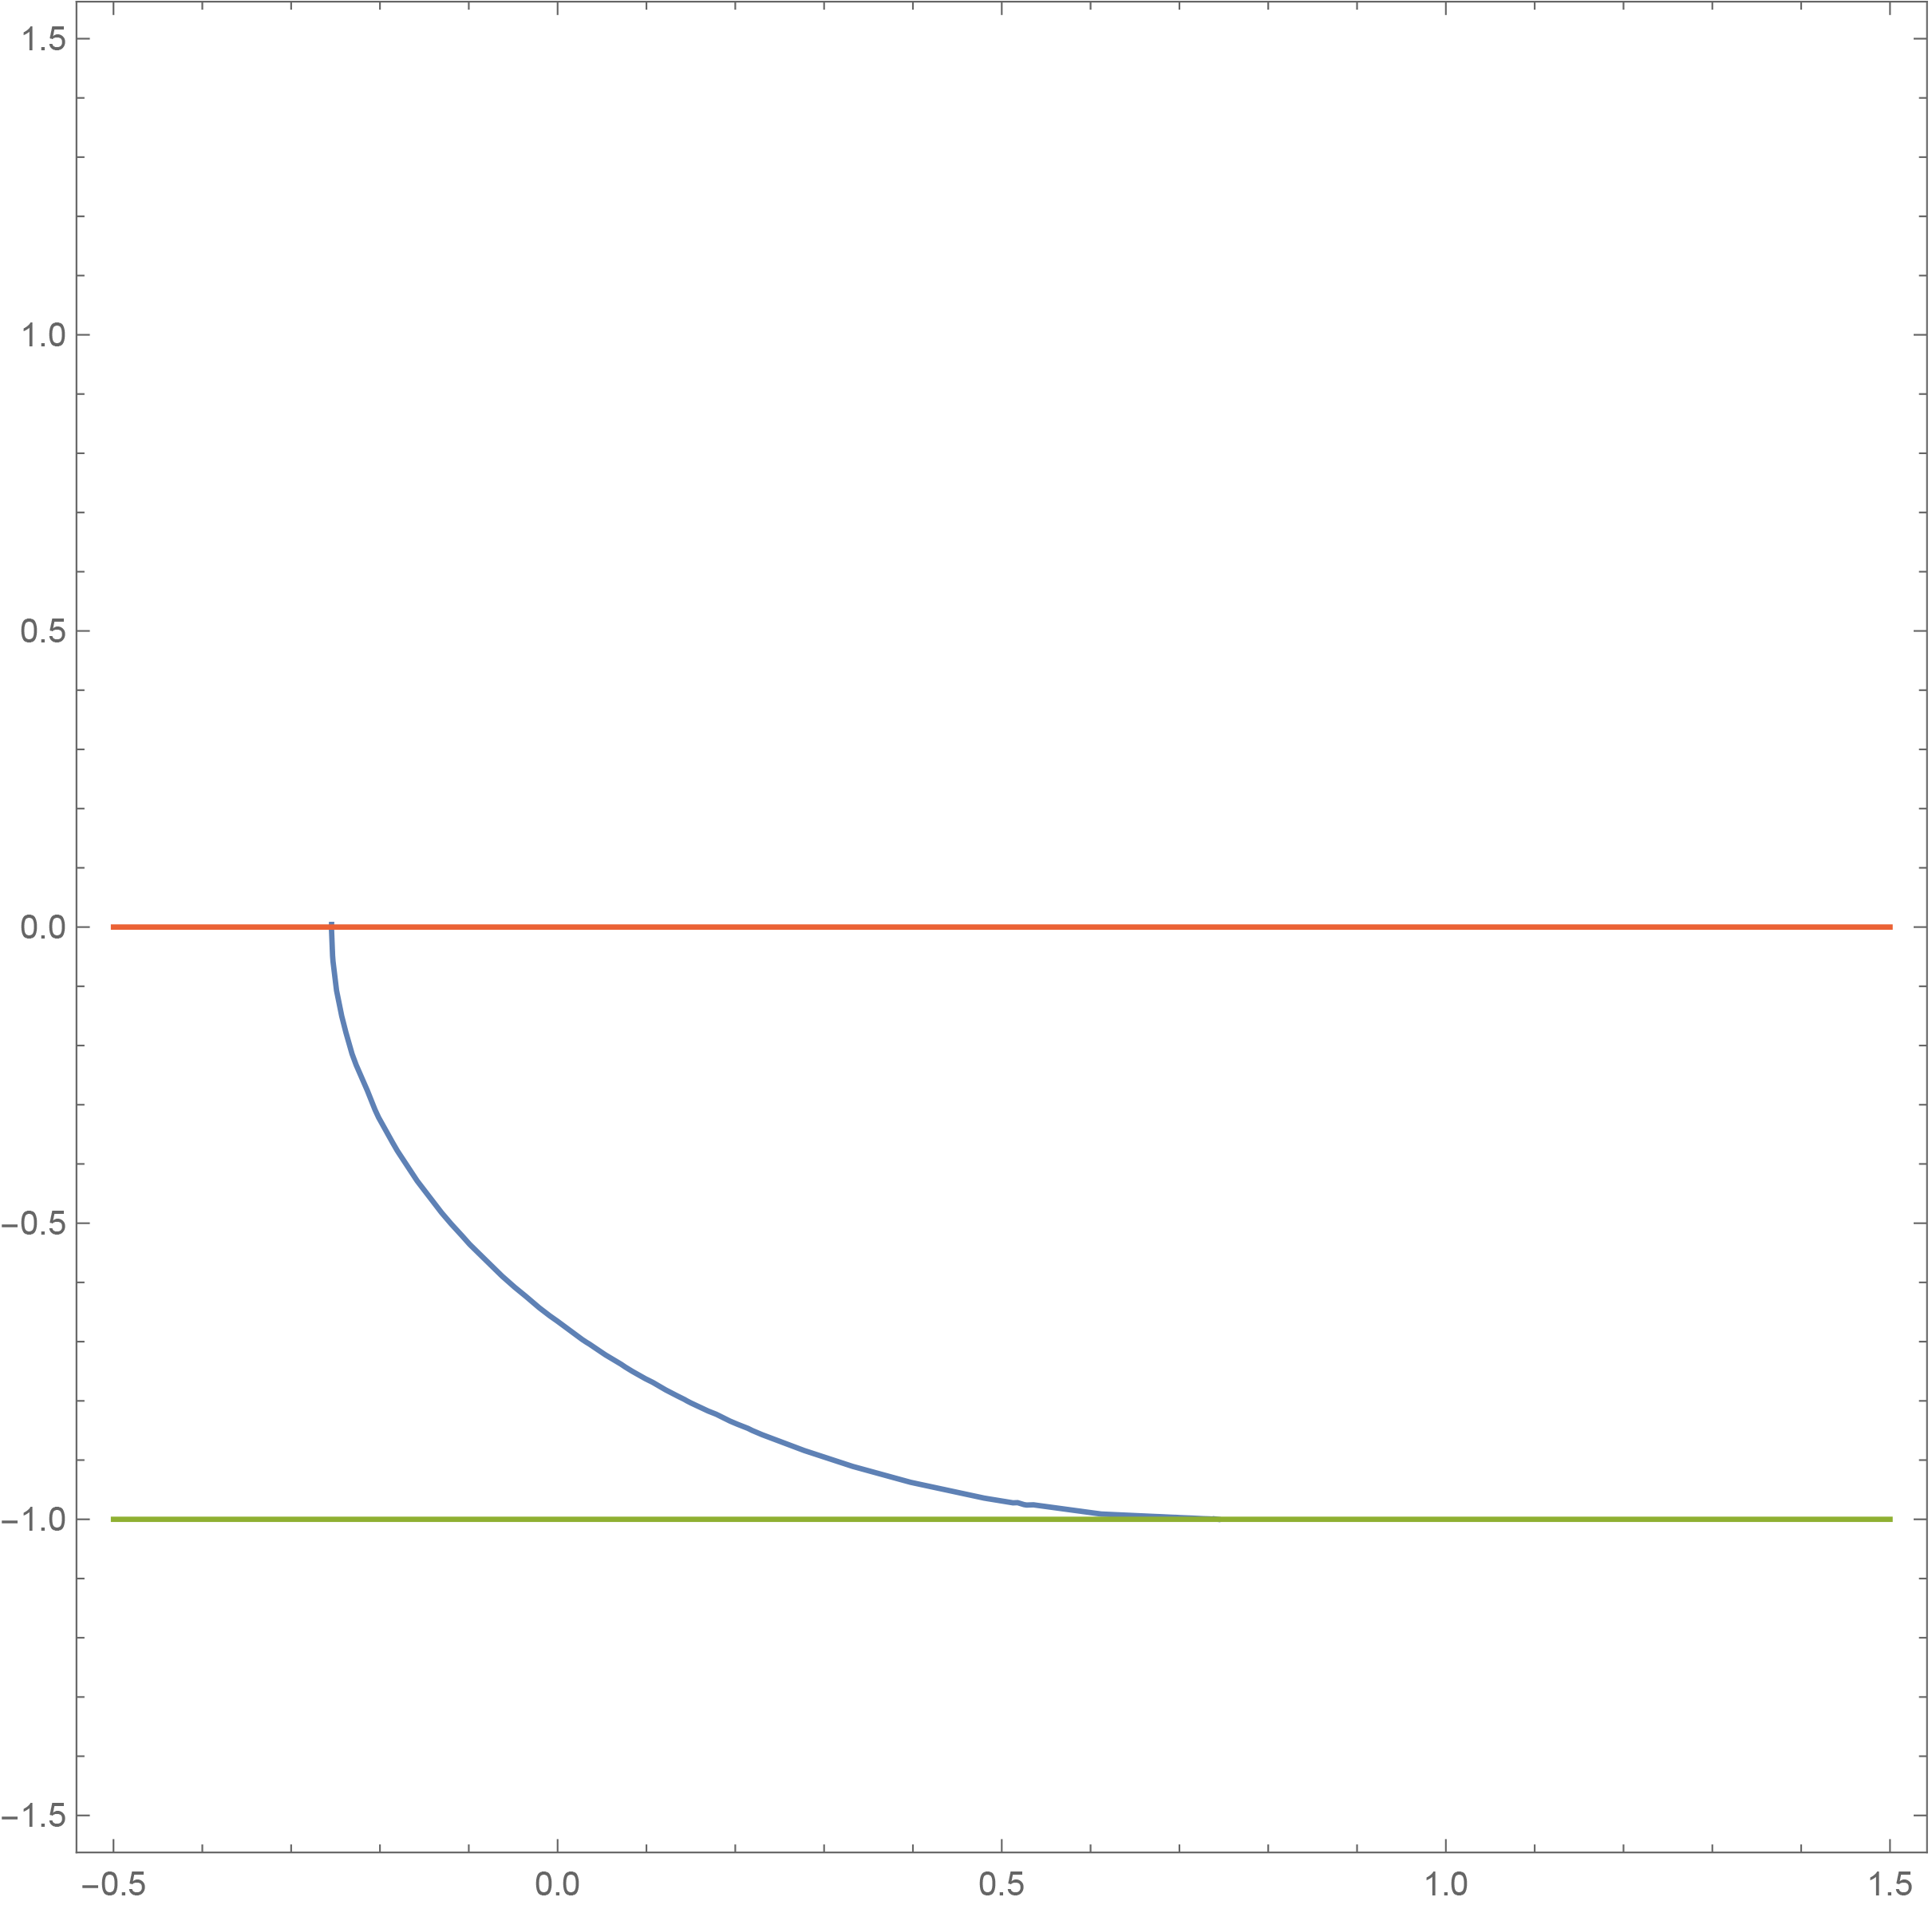
\includegraphics[scale=0.47]{3.png}
	\caption{Решение ДУ (1) с учетом начальных условий $(0, -2/3)$}
\end{figure}


	\subsection {Задача 2}

Задача Коши 
\begin{equation}
	y'-xy=e^{x},\;\;\;\;\;\;y(1) = 1, \;\;\;\;\;\;y(\cdot) \in \bf{R}
\end{equation}
Решение полностью аналогично решению №2 варианта I.


\[v= e^{\frac{x^2} 2}\]
\[u=\int_{1}^x e^{-s^2/2+s} ds+ c= e^{1/2} \int_{1}^{x} e^{-s^2/2-s+1/2} ds+c = e^{1/2}\int_0^{(x-1)} e^{-t^2/2} dt+c\]
\[y = uv = e^{\frac{x^2} 2}  e^{1/2}\int_{0}^{(x-1)} e^{-t^2/2} dt+ce^{\frac{x^2} 2}\] 
Найдем константу:
\[y(1)=ce^{1/2}=1\;\;\;\;\;\; c = e^{-1/2}\]
Тогда решение имеет вид:
\[y =e^{\frac{x^2} 2 + \frac 1 2 } \int_{0}^{(x-1)} e^{-t^2/2} dt+e^{\frac{x^2} 2 - \frac 1 2 }\] 

(iii) Предел на бесконечности:
\[ \lim_{x\rightarrow +\infty} e^{\frac{x^2} 2 + \frac 1 2 } \int_{0}^{(x-1)} e^{-t^2/2} dt+e^{\frac{x^2} 2 - \frac 1 2 } =\lim_{x\rightarrow +\infty} e^{\frac{x^2} 2 + \frac 1 2 }\sqrt{ \pi / 2 } +e^{\frac{x^2} 2 - \frac 1 2 } =+\infty \] т.к. интеграл стремится к $\sqrt{\pi/2} $

\[ \lim_{x\rightarrow -\infty} e^{\frac{x^2} 2 + \frac 1 2 } \int_{0}^{(x-1)/ } e^{-t^2/2} dt+e^{\frac{x^2} 2 + \frac 1 2 } =\lim_{x\rightarrow -\infty} - e^{\frac{x^2} 2 + \frac 1 2 } \sqrt{ \pi /2} +e^{\frac{x^2} 2 - \frac 1 2 } =-\infty \] т.к интеграл стремится к $-\sqrt{ \pi / 2}.$

(iv) График решения:\\
\begin{figure}[H]
	\centering
	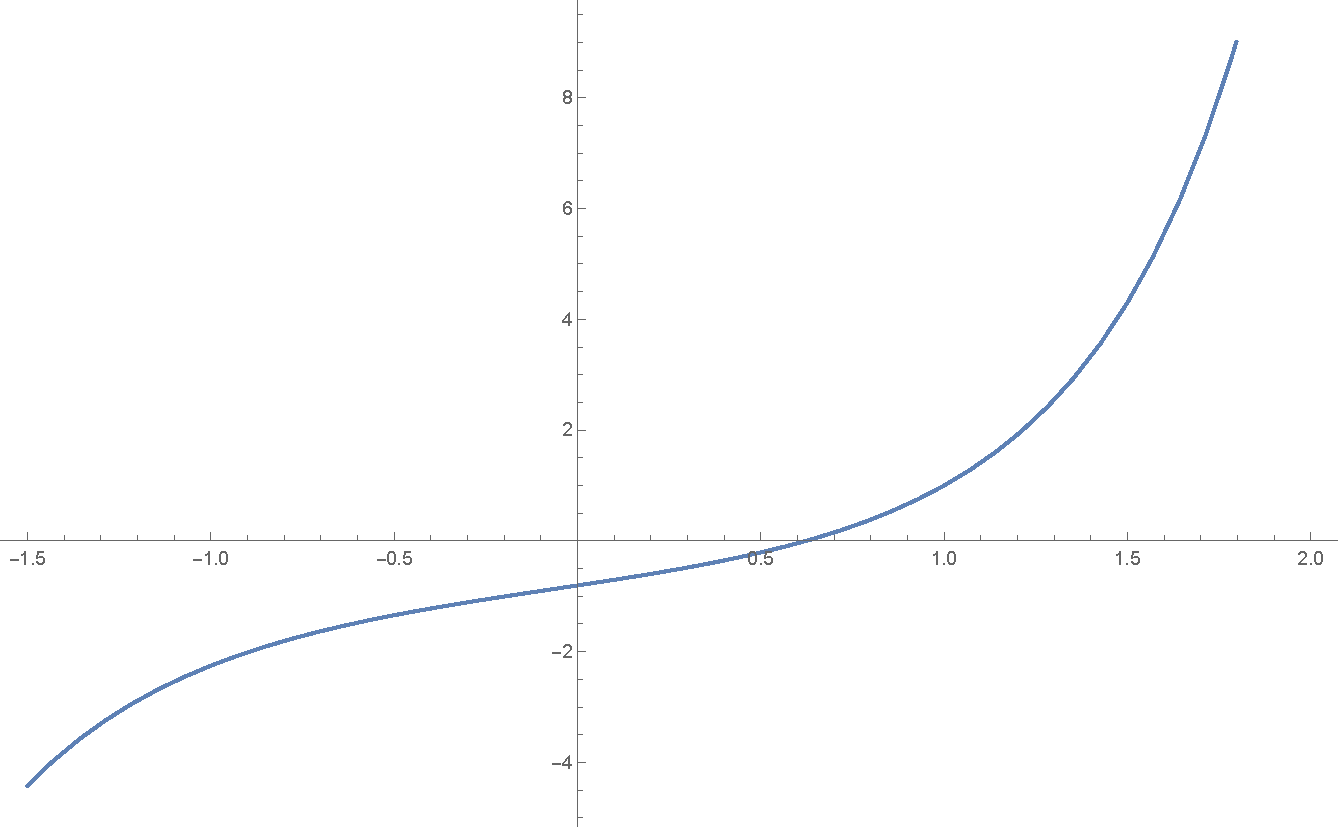
\includegraphics[scale=0.65]{15}
	\caption{Решение задачи Коши (9)}
\end{figure}

\begin{figure}[H]
	\centering
	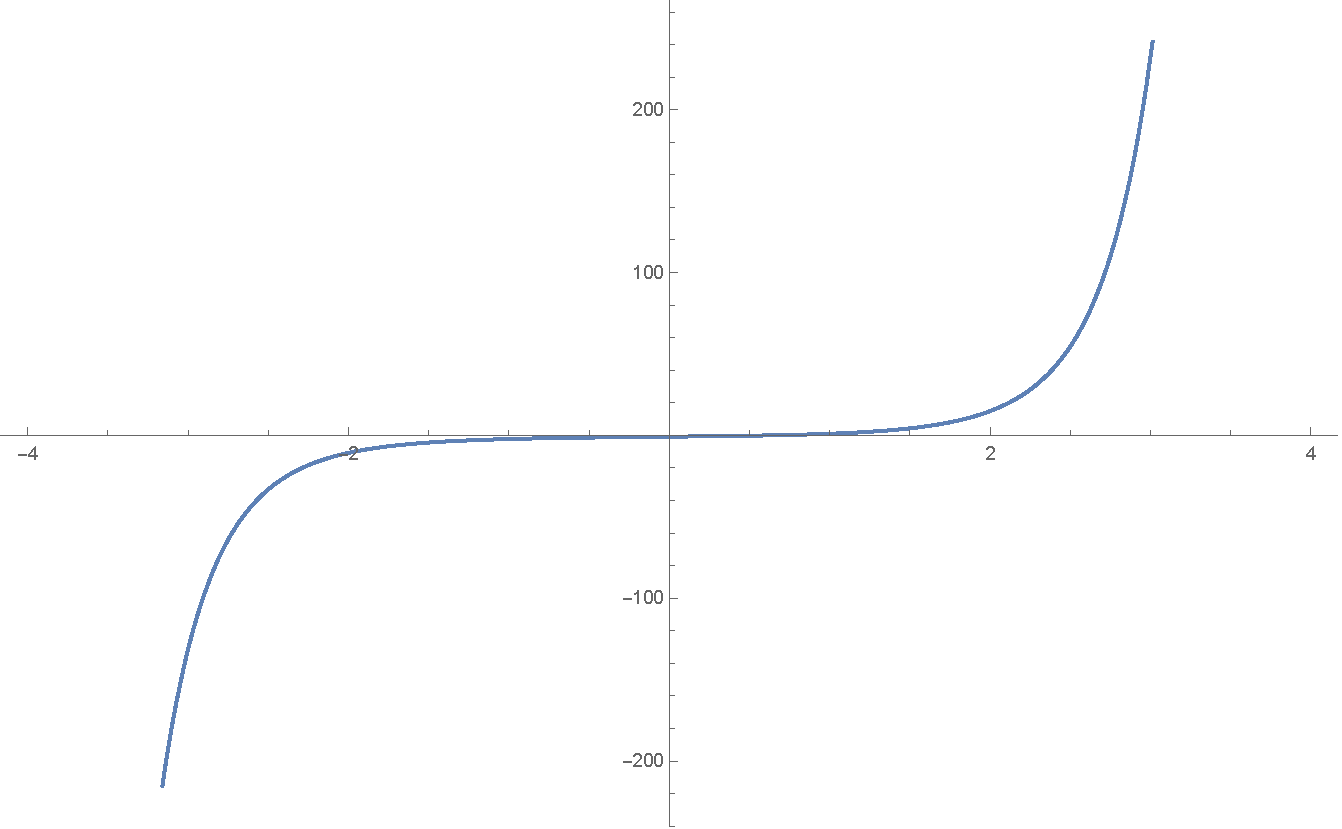
\includegraphics[scale=0.65]{14}
	\caption{Решение задачи Коши (9)}
\end{figure}


		\subsection {Задача 3}


\begin{equation}
\frac {dy}{dx}= - \frac {2y}{-x+y}, \;\;\;\;\; y(\cdot)\in \bf{R}
\end{equation}

(i) $D = R \times R \backslash \{y = x\}$. Производная правой части непрерывна на D -- решения всюду единственны. По т. Пеано решения существуют.\\ 

Найдем эти решения. Уравнение однородное:
\[y = u\cdot v,\;\;\;\;\;\;y'=u'v+uv'\]
\[v'u+vu'= - \frac{2vu}{vu-x}\]
Пусть
\[u = x\]
Тогда 
\[v'x= - \frac {v(v+1)}{v-1}\]
Разделяя переменные и интегрируя, получим:
\[2\ln(v+1)-\ln(v)=-\ln(x)+C\]
\[\frac{y}{x(y/x+1)^2} C= x\]
\[y = \frac {c-2x+\sqrt{c(-4x+c)}}{2}\]
\[y =\frac {c-2x-\sqrt{c(-4x+c)}}{2}\]
Из гранусловий находим, что 
\[c = 1\]
Тогда
\begin{equation}
y =\frac {1-2x+\sqrt{-4x+1}}{2}\;\;\text{ -- уравнение нашей кривой.}
\end{equation}


(ii) Максимальные интервалы существования решения:\\
Кривая проходит через точку (0, 1), следовательно, она монотонно убывает (см. пункт (iv)) до пересечения с прямой y=x, исключенной из D. Слева (11) ничем не ограничена. Тогда можем найти максимальный интервал существования решения: \[x \in (-\infty; 1/4)\]


(iii) Асимптотика на границах интервала существования.\\
\[\lim_{x\rightarrow 1/4} y(x) =1/4\]
\[y(x) = \frac {1-2x+\sqrt{-4x+1}}{2} = 1/2-x+O(x^{1/2}) \quad \quad \text{при $x \rightarrow - \infty$} \]
Асимптоты в этом случае нет. 


(iv) Монотонность и график решения:

Знаки производной:
\[y' > 0\;\;\;\;\; \frac y {x-y}>0\]
\[
\left[ 
  \begin{gathered} 
    \left\{ 
      \begin{gathered} 
        y  > 0
        \\ 
         x -  y > 0
        \\
      \end{gathered} 
    \right.  
    \\ 
    \left\{ 
      \begin{gathered} 
        y  < 0
        \\ 
        x - y < 0
        \\
      \end{gathered} 
    \right.
    \\
  \end{gathered}
\right.
\]

\begin{figure}[H]
	\centering
	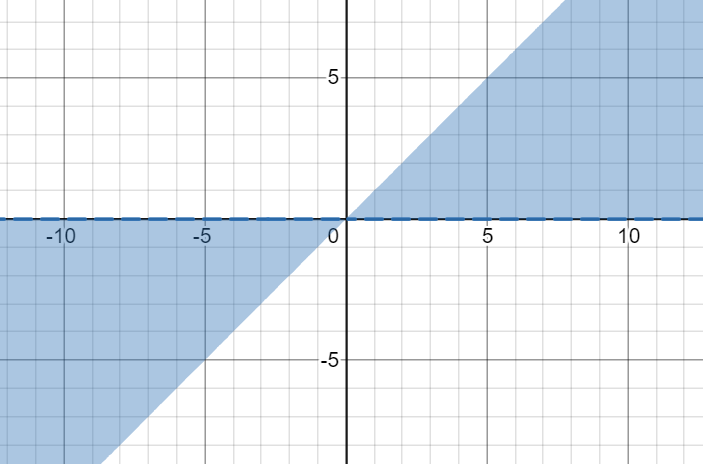
\includegraphics[scale=0.7]{10}
	\caption{Знаки производной (производная положительна в закрашенной области)}
\end{figure}

Решение (10) монотонно убывает на $(-\infty; 1/4)$.

Наше решение проходит через точку $(0, 1)$ на плоскости, следовательно, наша траектория убывает и втыкается в прямую y=x, не входящую в D. 

Рассмотрим поведение производной на правой границе:
\[\lim_{x\rightarrow y} y'(x) =-\infty\]
Кривая почти вертикально входит в $y=x.$

\begin{figure}[H]
	\centering
	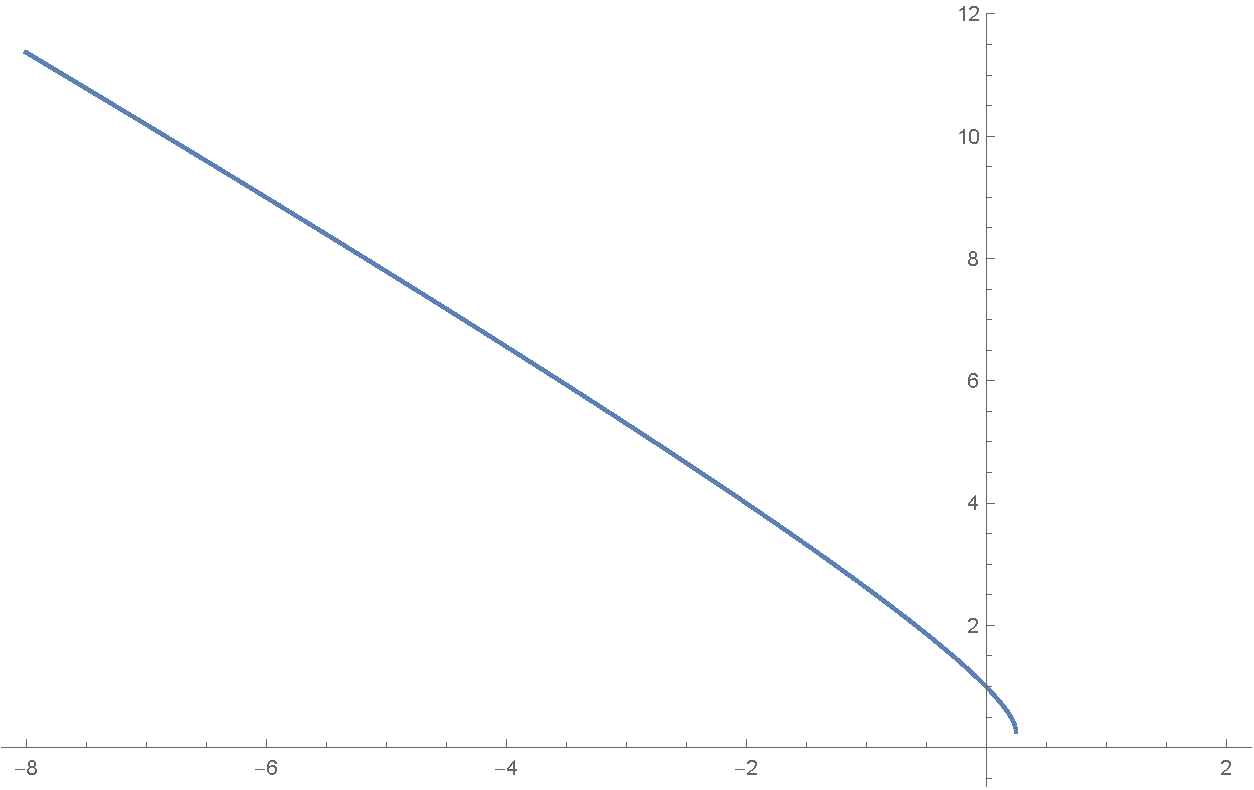
\includegraphics[scale=0.7]{8}
\caption{Решение задачи Коши (10) с условием $(0, 1)$)}
\end{figure}


\end{document}